\documentclass[t,table,usenames,dvipsnames]{beamer}

\usetheme{CambridgeUS}
\usecolortheme{beaver}
\setbeamertemplate{navigation symbols}{}

\usepackage[utf8]{inputenc}
\usepackage[croatian]{babel}

\usepackage{datetime}
\renewcommand{\dateseparator}{.}
\newcommand{\todayiso}{\twodigit\day \dateseparator \twodigit\month \dateseparator \the \year}
\date{\todayiso}

\usepackage{listing}
\usepackage{graphicx}
\usepackage{subcaption}
\usepackage{multirow}
\usepackage{color}
\definecolor{LightGray}{gray}{0.9}
\captionsetup{compatibility=false}

\title[NKOSL]{Napredno korištenje operacijskog sustava Linux}
\author[Dominik Barbarić]{Dominik Barbarić\\{\small Nositelj: doc.dr.sc. Stjepan Groš}}
\subtitle{3. Mreže}
\institute[FER]{Sveučilište u Zagrebu\\Fakultet elektrotehnike i računarstva}

\begin{document}

{
	\setbeamertemplate{footline}{}
	\begin{frame}
		\maketitle
	\end{frame}
}

\begin{frame}
	\frametitle{Sadržaj}
	\tableofcontents
\end{frame}

\section{TCP/IP model}

\begin{frame}
	\frametitle{Modeli mreža}
	\centering
	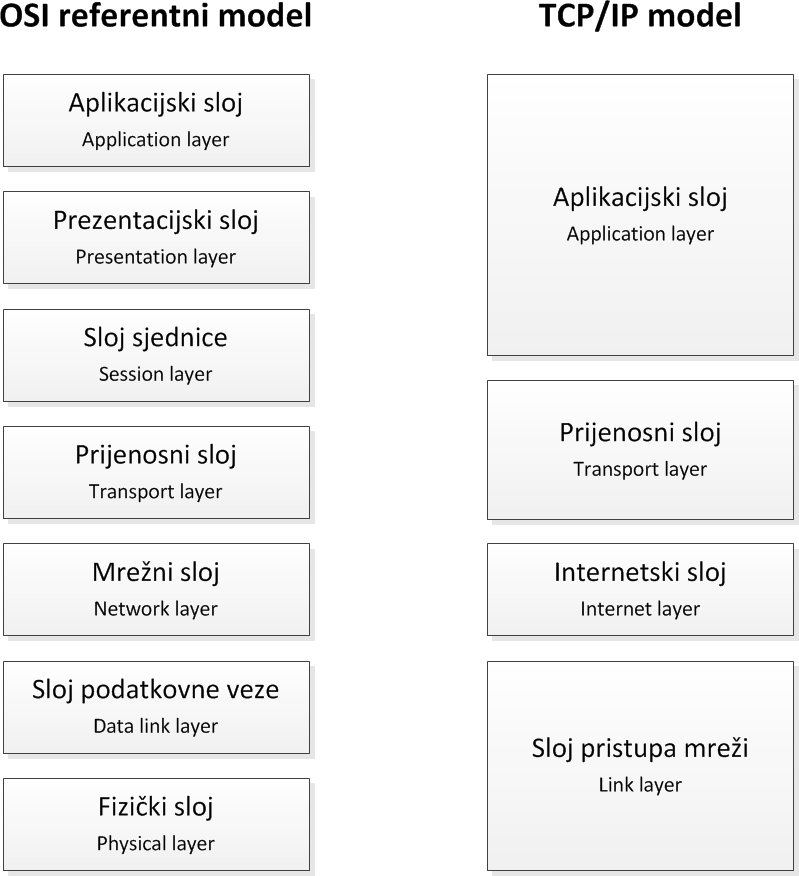
\includegraphics[width=0.55\textwidth]{osi_tcpip.png}
\end{frame}

\begin{frame}
	\frametitle{Modeli mreža}
	Internet
	\begin{itemize}
		\item Koristi TCP/IP model
		\item \textbf{Globalna mreža}
		\begin{itemize}
			\item Komutacija paketa
		\end{itemize}
	\end{itemize}
	\vfill
	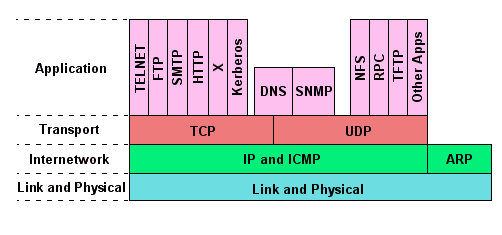
\includegraphics[width=0.8\textwidth]{service_layer.png}
\end{frame}

\begin{frame}
	\frametitle{Adresiranje u TCP/IP modelu}
	\textbf{Sloj pristupa mreži}
	\begin{itemize}
		\item Različito implementiran za svaku metodu pristupa (Ethernet, WLAN, \dots)
		\item \textbf{MAC (Media Access Control)}
		\begin{itemize}
			\item Osigurava pristup mediju, tj. dijelu mreže s kojom je uređaj izravno povezan
			\item Svaki mrežni uređaj ima jedinstvenu (hardversku) \emph{MAC adresu} oblika
			\item[] \texttt{0a:1b:2c:3d:4e:5f} \hfill (48b u hex zapisu) \hfill \,
		\end{itemize}
		\item MAC protokol omogućuje komutaciju paketa među izravno povezanim uređajima
	\end{itemize}
\end{frame}

\begin{frame}
	\frametitle{Adresiranje u TCP/IP modelu}
	\textbf{Internetski sloj}
	\begin{itemize}
		\item Omogućuje komutaciju na velikoj mreži
		\item Adresiranje \emph{IP adresom} oblika
		\item[] \texttt{192.168.100.100} \hfill (IPv4 - 32b u dec zapisu) \hfill \,
	\end{itemize}
	Subnet
	\begin{itemize}
		\item Podmreža koja koristi raspon IP adresa odvojen od ostatka mreže
		\item Podmreža koristi raspon određen IP adresom mreže i \emph{subnet mask}om
		\item Pristup ostalim mrežama ostvaruje se \emph{routing}om
	\end{itemize}
	\begin{itemize}
		\item Rasponi rezervirani za lokalne mreže
		{\ttfamily
			\item[] 10.0.0.0/8
			\item[] 172.16.0.0/12
			\item[] 192.168.0.0/16
		}
		
	\end{itemize}
\end{frame}

\begin{frame}[fragile]
	\frametitle{Adresiranje u TCP/IP modelu}
	\framesubtitle{Primjer određivanja subneta}
	\footnotesize
	Mreža je određena adresom mreže i subnet maskom
	\begin{verbatim}
Network: 172.16.64.0
Mask:    255.255.192.0
	\end{verbatim}
	Subnet mask se raspisom u binarni oblik može zapisati:
	\begin{verbatim}
         11111111.11111111.11000000.00000000
	\end{verbatim}
	Na isti način adresa mreže se može zapisati:
	\begin{verbatim}
         10101100.00010000.01000000.00000000
	\end{verbatim}
	Pozicija na kojoj u subnet masku stoji \texttt{1} je fiksirana i taj bit IP adrese je nepromjenjiv unutar subneta. Stoga su u subnetu moguće IP adrese oblika:
	\begin{verbatim}
         10101100.00010000.01******.********
	\end{verbatim}
	U decimalnom zapisu:
	\begin{verbatim}
         172.16.64.0 - 172.16.127.255
	\end{verbatim}
\end{frame}

\begin{frame}[fragile]
	\frametitle{Adresiranje u TCP/IP modelu}
	\begin{verbatim}
	Network: 172.16.64.0
	Mask:    255.255.192.0
	\end{verbatim}
	\begin{itemize}
		\item CIDR notacijom adresa mreže se zapisuje u obliku
		\item[] \texttt{172.16.64.0/18}
	\end{itemize}
	\begin{itemize}
		\item Broj iza adrese mreže odgovara broju mjesta na kojima u subnet masku stoji \texttt{1}
	\end{itemize}
\end{frame}

\subsection{IP konfiguracija}
\begin{frame}
	\frametitle{Konfiguracija mreže}
	\begin{itemize}
		\item IP adresa se dodjeljuje
		\begin{itemize}
			\item Dinamički - DHCP protokol
			\item Statički
		\end{itemize}
		\item Konfiguracija se obavlja kroz
		\begin{itemize}
			\item \texttt{/etc/network/interfaces}
			\item systemd-networkd
			\item NetworkManager
		\end{itemize}
	\end{itemize}
\end{frame}

\begin{frame}[fragile]
	\frametitle{Konfiguracija mreže}
	\framesubtitle{\texttt{/etc/network/interfaces}}
	\vspace{-1em}
	\begin{verbatim}
auto eth0
iface eth0 inet static
address 192.168.1.5
netmask 255.255.255.0
gateway 192.168.1.254

auto eth1
iface eth1 inet dhcp
	\end{verbatim}
	\begin{itemize}
		\item \texttt{auto eth0} - \texttt{eth0} se omogućuje pri startupu
		\item \texttt{iface eth0 inet static} - \texttt{eth0} ima dodijeljenu statičku IP adresu
		\item \texttt{iface eth1 inet dhcp} - \texttt{eth1} traži dinamičku IP adresu
	\end{itemize}
\end{frame}

\begin{frame}
	\frametitle{Konfiguracija mreže}
	\begin{itemize}
		\item \texttt{/etc/network/interfaces} se čita prilikom pokretanja \emph{networking} servisa
		\item[] \texttt{/etc/init.d/networking restart}
	\end{itemize}
	\begin{itemize}
		\item Neke naredbe za promjenu konfiguracije
	\end{itemize}
	\begin{table}[h]
		\rowcolors{1}{White}{LightGray}
		\begin{tabular}{p{4cm} p{3cm} p{3cm}}
			\rowcolor{BlueViolet!20}Operacija & \texttt{ifconfig} & \texttt{ip} \\
			Pregled konfiguracije & \texttt{ifconfig} & \texttt{ip addr show} \\ & & \texttt{ip link show} \\
			Uključenje i isključenje sučelja & \texttt{ifconfig <interface> up|down} & \texttt{ip link set <interface> up|down} \\
			Podešavanje IP adrese & \texttt{ifconfig <interface> <IP>} & \texttt{ip address add|del <IP> dev <interface>}
		\end{tabular}
	\end{table}
\end{frame}

\begin{frame}
	\frametitle{Konfiguracija mreže}
	\framesubtitle{NetworkManager}
	
	\begin{figure}[h]
		\begin{minipage}{0.4\textwidth}
			\centering
			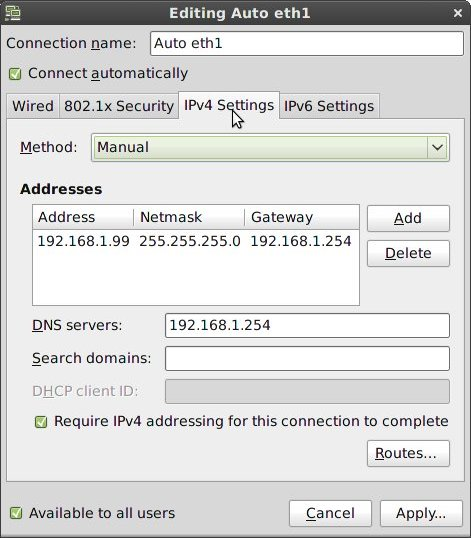
\includegraphics[width=\linewidth]{nm-ethernet.jpg}
			\caption*{Konfiguracija IP adrese}
		\end{minipage}
		\begin{minipage}{0.45\textwidth}
			\centering
			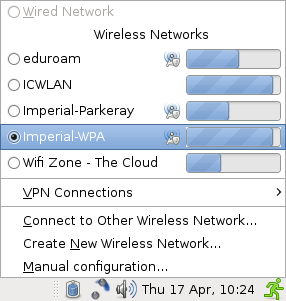
\includegraphics[width=0.8\linewidth]{nm-applet.png}
			\caption*{Odabir WLAN mreže}
		\end{minipage}
	\end{figure}
\end{frame}

\subsection{Routing}
\begin{frame}[fragile]
	\frametitle{Routing}
	\begin{itemize}
		\item Povezivanje subneta ostvaruje se \emph{routing}om
		\item Računalo ima konfigurirane rute preko kojih ostvaruje povezanost sa drugim mrežama
	\end{itemize}
	\begin{itemize}
		\item Rute su određene odredišnom adresom i adresom routera ili gatewaya
	\end{itemize}
	{\footnotesize \begin{verbatim}
# route -n
Kernel IP routing table
Destination   Gateway       Genmask        Flags Metric Ref  Use Iface
192.168.1.0   0.0.0.0       255.255.255.0  U     0      0      0 eth0
10.0.0.0      192.168.1.2   255.0.0.0      UG    1      0      0 eth0
0.0.0.0       192.168.1.10  0.0.0.0        UG    0      0      0 eth0

# ip route show
192.168.99.0/24 dev eth0  scope link
10.0.0.0/8 via 192.168.1.2  scope link  dev eth0  metric 1
default via 192.168.1.10 dev eth0
	\end{verbatim} }
\end{frame}

\subsection{DNS}
\begin{frame}[fragile]
	\frametitle{DNS}
	\begin{itemize}
		\item Prevođenje imena računala (tekstualne adrese) u IP adresu
	\end{itemize}
	\begin{verbatim}
    $ dig www.fer.hr
    www.fer.hr.    3600   IN   A   161.53.72.119
	\end{verbatim}
	\begin{itemize}
		\item Popis DNS servera u \texttt{/etc/resolv.conf}
	\end{itemize}
	\begin{verbatim}
    nameserver 8.8.8.8
    nameserver 8.8.4.4
	\end{verbatim}
	\begin{itemize}
		\item Kod dinamičke konfiguracije DHCP server dojavljuje popis DNS servera
	\end{itemize}
\end{frame}

\section{iptables}
\begin{frame}
	\frametitle{iptables}
	\textbf{iptables}
	\begin{itemize}
		\item Firewall na Linuxu
		\item \emph{Netfilter} framework u kernelu
	\end{itemize}
	
	\begin{itemize}
		\item Provjerava, mijenja, prosljeđuje ili odbacuje pakete prema pravilima u tablici
		\item Tablica se sastoji od lanaca (\emph{chains}), a lanci od pravila (\emph{rules})
		\item Svako pravilo je definirano oblikom paketa na koji se odnosi i akcijom koju obavlja nad tim paketom (\emph{target})
	\end{itemize}
\end{frame}

\begin{frame}
	\frametitle{iptables}
	\centering
	\vspace{-1em}
	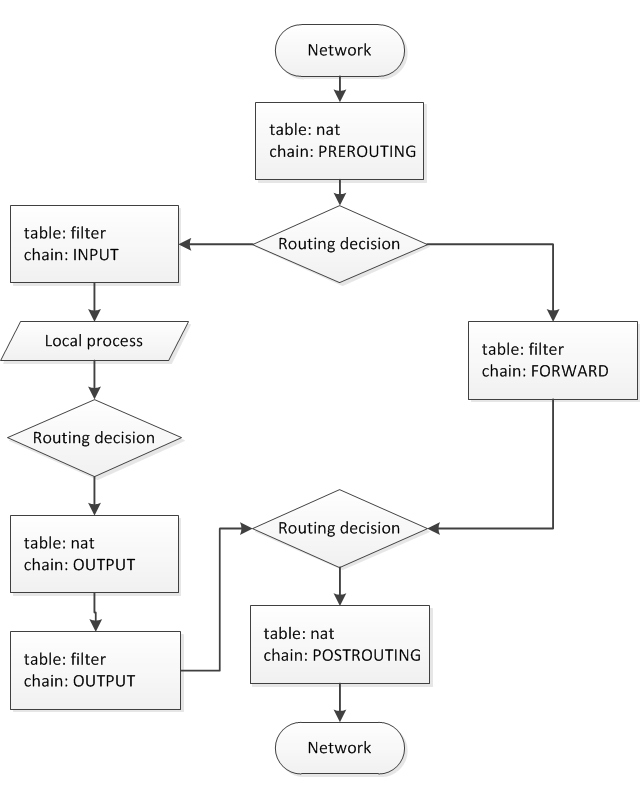
\includegraphics[width=0.5\textwidth]{iptables.png}
\end{frame}

\section{WLAN}
\begin{frame}
	\frametitle{WLAN}
	\begin{itemize}
		\item 802.11 a/b/g/n
	\end{itemize}
	Bežićna mreža je određena s
	\begin{itemize}
		\item SSID - naziv mreže
		\item BSSID - identifikator AP-a
		\item Sigurnosna razina
		\begin{itemize}
			\item Otvorena mreža
			\item WEP
			\item WPA - Personal i Enterprise
		\end{itemize}
	\end{itemize}
\end{frame}

\begin{frame}
	\frametitle{Podešavanje pristupa mreži}
	\framesubtitle{Pregled naredbi}
	\begin{table}[h]
		\rowcolors{1}{LightGray}{White}
		\begin{tabular}{l l}
			Pretraživanje mreža & \texttt{iwlist scan wl0}\\
			Odabir mreže (ESSID) & \texttt{iwconfig wl0 essid Ne\_kradi}\\
			Odabir mreže (SSID) & \texttt{iwconfig wl0 ap 00:11:22:33:44:55}\\
			& \texttt{iwconfig wl0 any}\\
			
			Spajanje na WEP mrežu & \texttt{iwconfig wlan0 essid}\\
			\hspace{1em} (hex ključ) & \hspace{1em} \texttt{Ne\_kradi key 0123456789}\\
			
			Spajanje na WEP mrežu & \texttt{iwconfig wlan0 essid}\\
			\hspace{1em} (string ključ) & \hspace{1em} \texttt{Ne\_kradi key s:password}
			
		\end{tabular}
	\end{table}
	
	\begin{itemize}
		\item Nakon spajanja na bežičnu mrežu slijedi uobičajena IP konfiguracija
		\item Za WPA mreže koristi se \texttt{wpa\_supplicant}
	\end{itemize}
\end{frame}

\begin{frame}[fragile]
	\frametitle{WLAN}
	\framesubtitle{wpa\_supplicant}
	\begin{itemize}
		\item Konfiguracija kroz \texttt{wpa\_cli} ili izravno \texttt{/etc/wpa\_supplicant.conf}
	\end{itemize}
	{\tiny \begin{verbatim}
$ wpa_passphrase MYSSID passphrase
network={
    ssid="MYSSID"
    #psk="passphrase"
    psk=59e0d07fa4c7741797a4e394f38a5c321e3bed51d54ad5fcbd3f84bc7415d73d
}
	\end{verbatim}
	\begin{block}{/etc/wpa\_supplicant/eduroam.conf}
	\begin{verbatim}
network={
   ssid="eduroam"
   proto=WPA2 WPA
   key_mgmt=WPA-EAP
   pairwise=CCMP TKIP
   group=CCMP TKIP
   ca_cert="<path_to_cert>/eduroam_fer.hr_CA.pem"
   subject_match="freeradius.fer.hr"
   identity="<USER>"
   eap=TTLS
   password="<PASSWORD>"
   phase2="auth=PAP"
}
	\end{verbatim}
	\end{block}}
\end{frame}

\section*{}
\begin{frame}
	\frametitle{Literatura}
	\footnotesize
	\url{https://wiki.debian.org/NetworkConfiguration}\\
	\url{https://wiki.archlinux.org/index.php/Network_configuration}
	\vfill
	\url{https://wiki.archlinux.org/index.php/iptables}\\
	\url{https://wiki.archlinux.org/index.php/Simple_stateful_firewall}
	\vfill
	\url{https://wiki.archlinux.org/index.php/Wireless_network_configuration}\\
	\url{https://wiki.archlinux.org/index.php/WPA_supplicant}
	\vfill
\end{frame}

\end{document}
